\chapter{Triggers}\label{sec:triggers}

%We are using the triggers in Table~\ref{triggertable} for the analysis with 19.4 fb$^{-1}$ of data. 

For the \tlth final states, we use single lepton triggers instead of
$l\times\tau_{h}$ cross-triggers to maintain a similar strategy across
channels and also allow us to use the $\tau_{h}$ isolation sidebands
as control and validation samples. For the \tetm final state, any
trigger with iso-muon requirement, either a e-$\mu$ cross-trigger or
single-muon trigger, would eliminate the isolation sideband for QCD
estimation. Hence, we use the same single-electron trigger as for the
\teth final state. Trigger paths are summarized in
Table~\ref{tab:triggernames}. Note this constrains the object ID and
phase space that we are studying. For example, the use of these
triggers requires $p_{T}$ cuts of 30 GeV, 35 GeV, and 60 GeV for our
leading light leptons and $\tau_{h}$'s in the \tmth, \teth, and \thth
channels, respectively.


\begin{table}[ht]
\begin{center}
  \caption{The trigger paths used to collected the data.  Emulated
    trigger paths, in particular those most similar to the paths used
    to collect the data, are applied to the simulated
    samples.\label{tab:triggernames}}
  \begin{tabular}{| l | c |}
  \hline
       Channel                & Trigger Path                                   \\[0.5ex] \hline
       \thth (data RunC, sim) & HLT\_DoubleMediumIsoPFTau40\_Trk1\_eta2p1\_Reg \\
       \thth (data RunD)      & HLT\_DoubleMediumIsoPFTau35\_Trk1\_eta2p1\_Reg \\ \hline
       \tmth (data RunC)      & HLT\_IsoMu24\_eta2p1                           \\
       \tmth (data RunD)      & HLT\_IsoMu18                                   \\
       \tmth (sim)            & HLT\_IsoMu17 (L1~$\mu\ \pt > 18\gev$)          \\ \hline
       \teth, \tetm (data)    & HLT\_Ele27\_eta2p1\_WPLoose                    \\
       \teth, \tetm (sim)     & HLT\_Ele27\_eta2p1\_WP75                       \\
  \hline
  \end{tabular}
\end{center}
\end{table}

\subsection{Single Lepton Trigger Efficiency}\label{sec:lepTrigger}
The single electron and muon trigger efficiencies are measured
using a tag and probe method where we selected events with at 
least one electron and one muon pair satisfying the following
requirements:

For electrons:
\begin{itemize}
  \item $p_T > 13~\gev$, $|\eta| < 2.1$, isolation $< 0.15$, $d_{xy}<0.045$~cm, $d_{z}<0.2$~cm
  \item passing electron ID (we performed different measurements for "MVANonTrigWP80", "HEEP", "MVATrigWP80")
  \item no matched conversions
  \item number of missing hits = 0
\end{itemize}

For muons:
\begin{itemize}
  \item $p_T > 20~\gev$, $|\eta| < 2.1$, isolation $< 0.15$, $d_{xy}<0.045$~cm, $d_{z}<0.2$~cm
  \item passing "Medium" muon ID
\end{itemize}

For the pair:
\begin{itemize}
  \item $\Delta$R(\tetm) $>$ 0.3
  \item choose the most isolated pair
  \item choose the opposite sign pair
  \item 3rd lepton veto
\end{itemize}

\subsection{Single Electron Trigger Efficiency}\label{sec:eleTrigger}
To measure the single-electron trigger efficiency, after the
preselection mentioned above, we select (tag) events with a
single-muon trigger (HLT\_IsoMu18 for data and HLT\_IsoMu17\_eta2p1
for MC with L1 $\mu~p_{T} > 18~\gev$) with the offline muon matching
the HLT muon that fired the trigger.  Then, the trigger efficiency is
defined at the fraction of events which also pass (probe) the
single-electron trigger (HLT\_Ele27\_eta2p1\_WPLoose for data and
HLT\_Ele27\_eta2p1\_WP75 for MC).

The efficiency curves of the single-electron triggers, measured
vs. electron \pt, are shown in Figure~\ref{fig:eturnon}. A
$p_{T}>35$~\gev cut is motivated to avoid the turn-on region. As shown
in Figure~\ref{fig:eturnon2}, the efficiency curves were further
binned into two $p_T$ bins containing similar numbers of events.  A
weight of 0.94 is measured, and used in the analysis, as the ratio
between simulated and observed events in which the selected electron
is in the endcap region.
\begin{figure}\centering
  \includegraphics[width=0.45\textwidth]{figures/et-em/triggerStudy/eleTrigTurnOnCurve_ePt_em_HEEP_barrel}
  \includegraphics[width=0.45\textwidth]{figures/et-em/triggerStudy/eleTrigTurnOnCurve_ePt_em_HEEP_endcap} \\
  \includegraphics[width=0.45\textwidth]{figures/et-em/triggerStudy/eleTrigTurnOnCurve_ePt_em_MVANonTrig80_barrel}
  \includegraphics[width=0.45\textwidth]{figures/et-em/triggerStudy/eleTrigTurnOnCurve_ePt_em_MVANonTrig80_endcap} \\
  \includegraphics[width=0.45\textwidth]{figures/et-em/triggerStudy/eleTrigTurnOnCurve_ePt_em_MVATrigWP80_barrel}
  \includegraphics[width=0.45\textwidth]{figures/et-em/triggerStudy/eleTrigTurnOnCurve_ePt_em_MVATrigWP80_endcap}
  \caption{\label{fig:eturnon} The efficiency vs. \pt curves of the
    single-electron triggers used.  Left column: barrel.  Right
    column: endcap.  The offline electron ID requirements used are
    HEEP (top row), MVANonTrig80 (middle row), MVATrigWP80 (bottom
    row).}
\end{figure}
\begin{figure}\centering
  \includegraphics[width=0.4\textwidth]{figures/et-em/triggerStudy_2bins/eleTrigTurnOnCurve_ePt_em_HEEP_barrel_2bins}
  \includegraphics[width=0.4\textwidth]{figures/et-em/triggerStudy_2bins/eleTrigTurnOnCurve_ePt_em_HEEP_endcap_2bins} \\
  \includegraphics[width=0.4\textwidth]{figures/et-em/triggerStudy_2bins/eleTrigTurnOnCurve_ePt_em_MVANonTrig80_barrel_2bins}
  \includegraphics[width=0.4\textwidth]{figures/et-em/triggerStudy_2bins/eleTrigTurnOnCurve_ePt_em_MVANonTrig80_endcap_2bins} \\
  \includegraphics[width=0.4\textwidth]{figures/et-em/triggerStudy_2bins/eleTrigTurnOnCurve_ePt_em_MVATrigWP80_barrel_2bins}
  \includegraphics[width=0.4\textwidth]{figures/et-em/triggerStudy_2bins/eleTrigTurnOnCurve_ePt_em_MVATrigWP80_endcap_2bins}
  \caption{\label{fig:eturnon2} The efficiency vs. \pt curves of the
    single-electron triggers used.  Left column: barrel.  Right
    column: endcap.  The offline electron ID requirements used are
    HEEP (top row), MVANonTrig80 (middle row), MVATrigWP80 (bottom
    row).  The two bins each contain half of the events with
    $\pt>35$~\gev.}
\end{figure}

\subsection{Single Muon Trigger Efficiency}\label{sec:muTrigger}
To measure the single-muon trigger efficiency, after the preselection
mentioned above, we select (tag) events with a single-electron trigger
 (HLT\_Ele27\_eta2p1\_WPLoose for data and HLT\_Ele27 \_eta2p1\_WP75 for MC) 
with the offline electron match the HLT electron that fired the trigger.
Then, the trigger efficiency is defined at the fraction of events
which also pass (probe) the single-muon trigger 
(HLT\_IsoMu18 for data and HLT\_IsoMu17\_eta2p1 for MC with L1 $\mu~p_T > $ 18 GeV).

The efficiency curves of the single-muon triggers, measured vs. muon
\pt, are shown in Figure~\ref{fig:muturnon}. A $\pt>25$~\gev cut is
motivated to avoid the turn-on region. As shown in lower two plots,
the efficiency curves were further binned into two bins containing
similar numbers of events.  Weights of 0.991 and 0.986 are measured,
and used in the analysis, as the ratios between simulated and observed
events in which the selected muon $|\eta| \leq 1.2$ and $|\eta|>1.2$.
\begin{figure}\centering
  \includegraphics[width=0.45\textwidth]{figures/et-em/triggerStudy/muonTrigTurnOnCurve_mPt_em_MVANonTrig80_mu_barrel}
  \includegraphics[width=0.45\textwidth]{figures/et-em/triggerStudy/muonTrigTurnOnCurve_mPt_em_MVANonTrig80_mu_endcap} \\
  \includegraphics[width=0.45\textwidth]{figures/et-em/triggerStudy_2bins/muonTrigTurnOnCurve_mPt_em_MVANonTrig80_mu_barrel_2bins}
  \includegraphics[width=0.45\textwidth]{figures/et-em/triggerStudy_2bins/muonTrigTurnOnCurve_mPt_em_MVANonTrig80_mu_endcap_2bins} \\
  \caption{\label{fig:muturnon} The efficiency vs. \pt curves of the
    single-muon triggers used.  Left column: $|\eta|<1.2$.  Right
    column: $|\eta|>1.2$.  Bottom row: the two bins each contain half
    of the events with $\pt>25$~\gev.}
\end{figure}

\subsection{Di-Tau Trigger Efficiency}\label{sec:tauTrigger}

The efficiency of the $\tau_{h}\tau_{h}$ trigger is measured using 
$Z\to\tau\tau\to\mu\tau_{h}$ events.  The $\tau_{h}$ candidates 
reconstructed in the selected $Z\to\tau\tau\to\mu\tau_{h}$ events are 
required to pass the same $\tau_{h}$ identification used for the final
analysis and which will be described in more detail in the sections to follow. The 
``denominator" selections used to define the $Z\to\tau\tau\to\mu\tau_{h}$ control sample 
are summarized below:

\begin{itemize}
  \item Events must fire the HLT{\_}IsoMu18 trigger ( HLT{\_}IsoMu17{\_}eta2p1 with HLT pt cut of 18 GeV for MC )
  \item $\ge 1$ global $\mu$ with $|\eta| < 2.1, p_{T} > 19$ GeV
  \item ``isMediumMuon"
  \item muon best track d$_{xy}$ $<$ 0.2~cm , d$_{z}$ $<$ 0.045~cm w.r.t. PV
  \item Relative isolation (with $\delta\beta$ corrections) $< 0.1$
  \item $\ge 1$ HPS $\tau_{h}$ with $|\eta| < 2.1, p_{T} > 20$ GeV
%  \item d$_{xy}$ w.r.t PV $<$ 0.2 , d$_{z}$ w.r.t PV $<$ 0.045 
  \item Muon veto: ``againstMuonTight3"
  \item Electron veto: ``againstElectronVLooseMVA5"
  \item ``old" decay mode finding %(1, 2, or 3 signal charged hadrons; see section 5)
  \item Isolation: ``byTightCombinedIsolationDeltaBetaCorr3Hits"
  \item p$_{T} >$ 5. GeV for leading Track of tau with d$_{xy} <$ 0.2~cm and d$_{z} <$ 0.045~cm w.r.t. PV
  \item $\Delta R(\mu,\tau_{h}) > 0.5$
  \item $Q(\mu) \times Q(\tau_{h}) < 0 $
  \item $m_{T}(\mu,\MET) < 40$ GeV
  \item 0 jets tagged as b-jets
  \item 0 tagged electrons
  \item veto events with a second muon forming opposite-sign dimuon pair
\end{itemize}\\\\

The numerator is defined by additionally requiring those events to 
pass the \\ 
HLT{\_}IsoMu17{\_}etap2p1{\_}MediumIsoPFTau40* trigger. 
The efficiency is measured for each $\tau_{h}$ leg individually and
parametrized as function of $p_{T}$ (Figure~\ref{fig:trigger}). From the 
plot it is clear that the emulation of the trigger in simulation does not 
provide the correct trigger efficiency observed in data. This is mainly 
due to a difference in the trigger definition in MC, specifically the 
L1 seed. Therefore, we do not apply the trigger in MC, but instead model 
the correct per leg trigger efficiency observed in data by weighing the 
predictions from simulation using the fit of the trigger efficiency 
curve in data (black solid curve in the plot). The trigger efficiency at 
the plateau is approximately 90\%. 
%comparison of the product of the per-leg trigger efficiency for the
%two legs in data and MC is applied as an event weight (0.95) to the MC
%events in order to match the trigger efficiency in data.

\begin{figure}[tbh!]
  \centering
    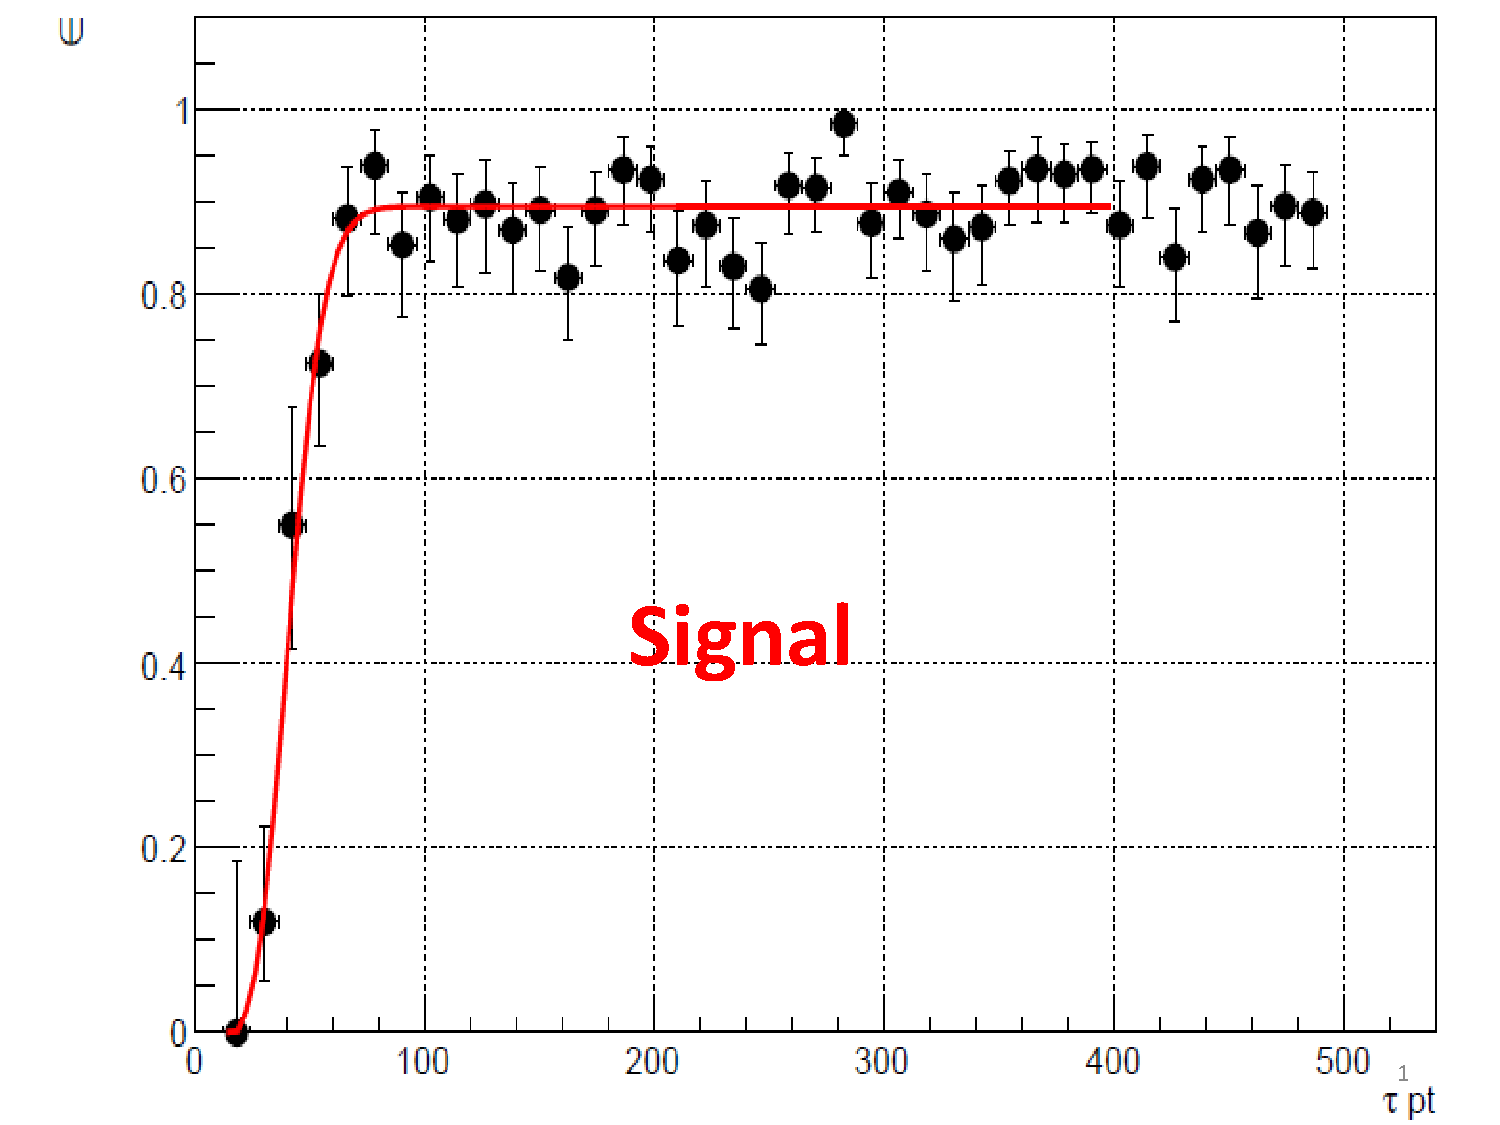
\includegraphics[width=0.4\textwidth]{TriggerEff_Signal.pdf}
    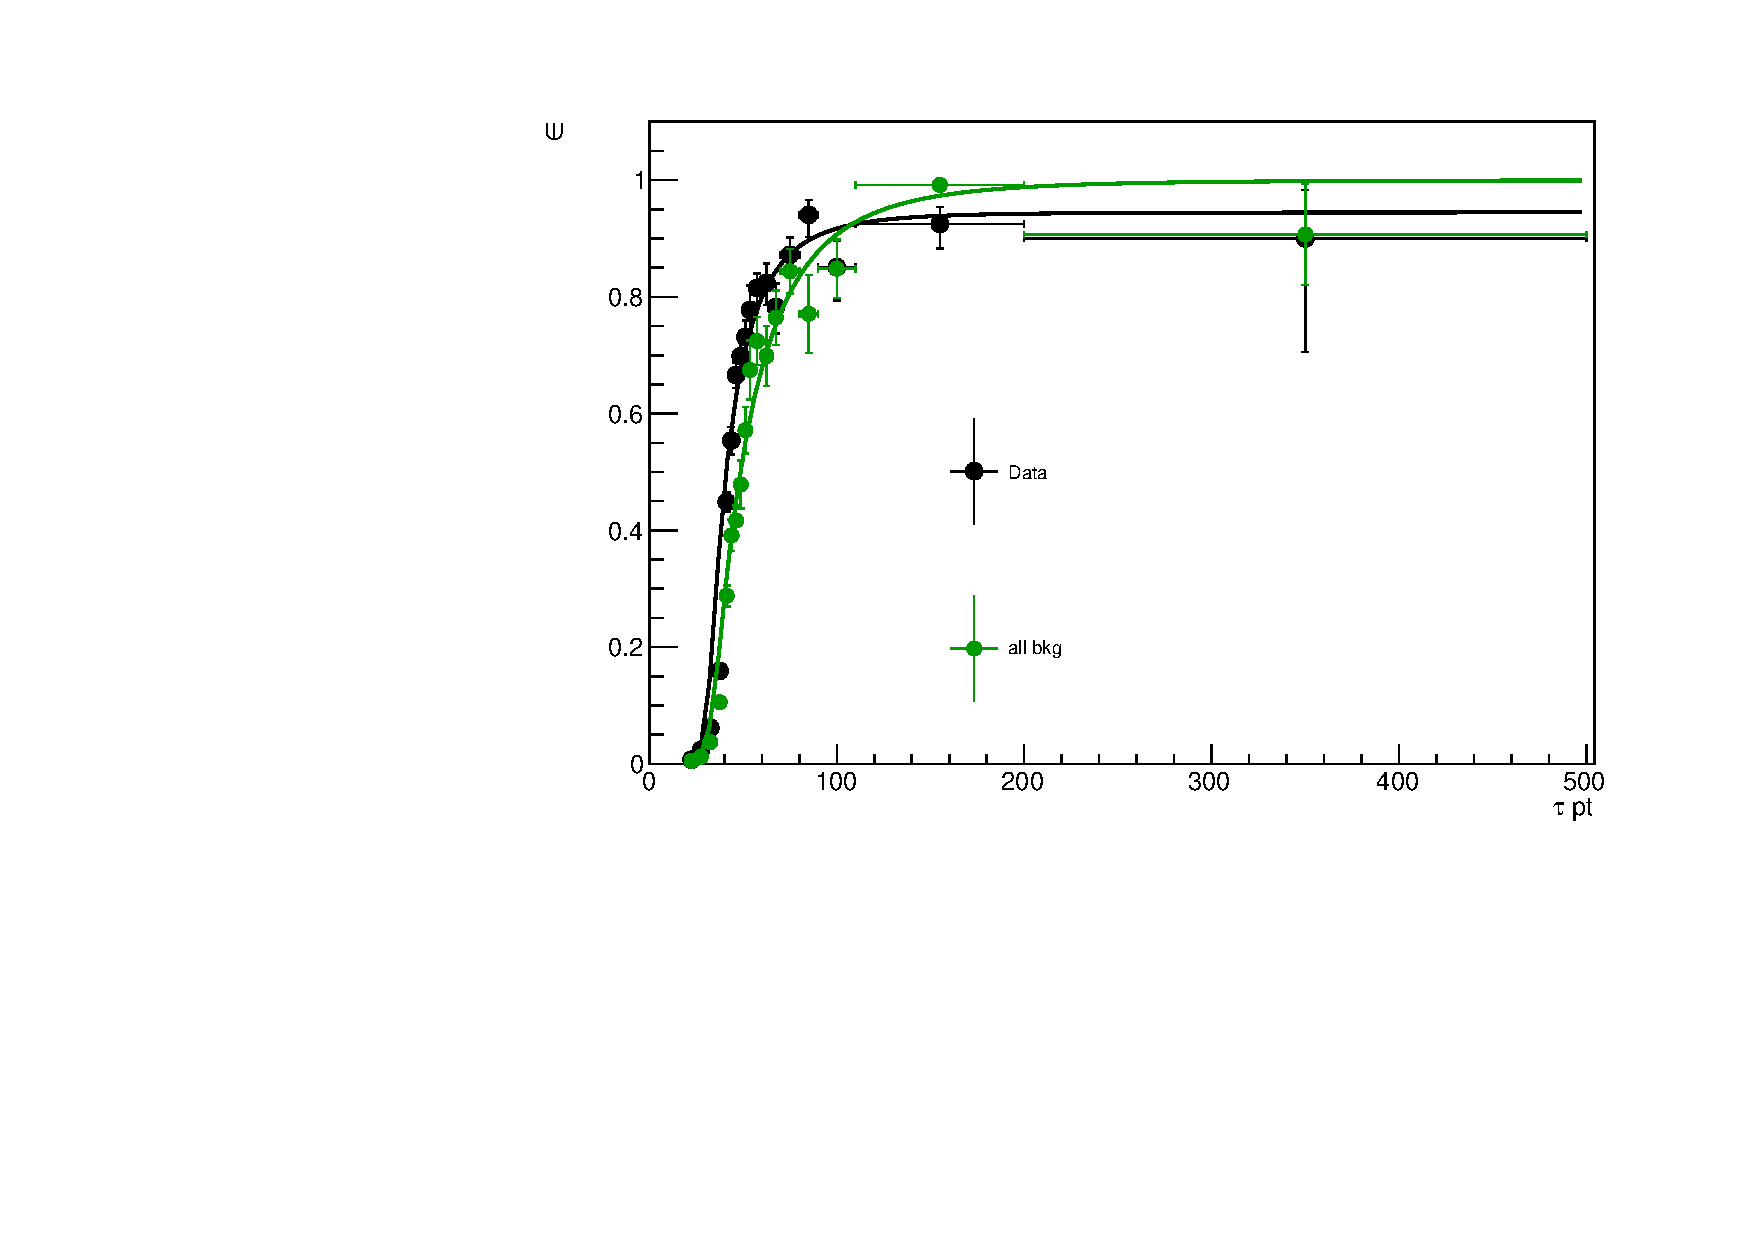
\includegraphics[width=0.5\textwidth]{CrystalBall.pdf}
  \caption{The per-leg $\tau_{h}$ trigger efficiency as a function of p$_{T}(\tau_{h})$ for (a) simulated Z$^{\prime}$ signal sample on left (b) for data and all backgrounds obtained by requiring mu-tau region on right.}
  \label{fig:trigger}
\end{figure}

Figure ~\ref{fig:trigger} (right) shows the trigger efficiency for data and all backgrounds obtained by requiring $Z\to\tau_{\mu} \tau_{h}$. Most of the backgrounds are taken from simulation except QCD whose shape and rate have been taken from same sign control region from data by subtracting the contribution of other backgrounds.QCD normalization is  then corrected by OS/LS ratio which is taken as $\sim$ 1.05. Table ~\ref{table:BGYieldtable} shows the event yield in this control region requiring the denominator selections. The ``purity", fraction of DYJets events out of all backgrounds, of this region comes out to be $\sim$ 65-66 \% . The efficiency curves on Figure ~\ref{fig:trigger} (right) is fitted with crystall-ball function.

\begin{table}[!htpb]
   \caption{Event rate in mu-tau control region after requiring denominator level selections }
   \centering{
    \begin{tabular}{| l | c |}
       \hline\hline
       Sample             & Events         \\ [0.5ex] \hline
       Data               &19578           \\
       t $\overline{t} $  &170.881$\pm$13.072          \\
       W+Jets           &2127.76$\pm$46.128          \\
       Z+Jets           &12218.5$\pm$110.544        \\
       QCD               &4003.93$\pm$63.277       \\
      \hline\hline
     \end{tabular}
   }        
   \label{table:BGYieldtable} % is used to refer this table in the text
 \end{table}
